\section[Social Media]{Social Media}

\begin{frame}{}
  \begin{center}
    \structure{\Large \insertsection}
  \end{center}
\end{frame}

\begin{frame}{Soziale Medien}
	\begin{columns}
	\column{150pt}
	\begin{itemize}
		\item <1-> Digitale Medien und Technologien um sich untereinander auszutauschen
		\item <2-> Heutzutage nicht mehr wegzudenken
		\item <3-> Viele verschiedene Optionen um in Kontakt zu bleiben
		\begin{itemize}
			\item <3-> Twitter
			\item <3-> Facebook
			\item <3-> Google+
			\item <3-> Foursquare
			\item <3-> ...
		\end{itemize}
	\end{itemize}
	\column{129pt}	
	\includegraphics<3->[height=4cm]{socialmedia-memes/facebook1.jpg}
	
	\end{columns}
\end{frame}

\begin{frame}
	\begin{itemize}
		\item <1->Wer sieht meine Einträge?
			
		\begin{itemize}
			\item <1->Abhängig vom Medium - ausgewählte Personen bis hin zu allen Teilnehmern eines Mediums
		\end{itemize}
			
		\item <2->Wem gehören meine Beiträge?
		\begin{itemize}
			\item <2-> Hängt von den jeweiligen Geschäftsbedingungen ab.
			\item <2-> z.B. Facebook: [...] nicht-exklusive, übertragbare, unterlizenzierbare, gebührenfreie, weltweite Lizenz zur Nutzung jeglicher IP-Inhalte, die du auf oder im Zusammenhang mit Facebook postest („IP-Lizenz“)[...]
		\end{itemize}
			
	\end{itemize}
\end{frame}

\begin{frame}
	\begin{columns}
	
	\column{150pt}	
	\begin{itemize}
		\item <1-> Was kann ich mit meinen Beiträgen machen?
		\begin{itemize}
			\item <2-> Kommt auf die jeweilige Plattform an
			\item <3-> Sehr problematisch, wenn Informationen an die falschen Leute gelangen.
		\end{itemize}
	\end{itemize}	
	\column{129pt}
	\includegraphics<4->[scale=0.5]{socialmedia-memes/scumbag_steve.jpg}
	\end{columns}
\end{frame}

\begin{frame}
	Was kann eigentlich alles schiefgehen? (Teil 1)\\
		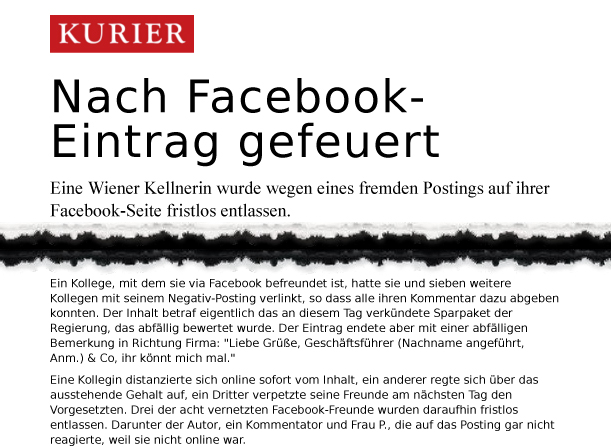
\includegraphics[scale=0.5]{facebook-news/facebook-gefeuert.jpg}
\end{frame}

\begin{frame}
	Was kann eigentlich alles schiefgehen? (Teil 2)\\
		
\includegraphics[scale=0.5]{facebook-news/facebook-party-200Bayern.jpg}
\end{frame}

\begin{frame}
	Was kann eigentlich alles schiefgehen? (Teil 3)
	\begin{itemize}
		\item Stalking
		\item Cyber-Mobbing
		\item Einbrüche (Foursquare weiß wo du bist!)
		\item Munition für (böswillige) Anwendungen, z.B. Girls Near Me
		\item Rechtliche Grauzonen!
	\end{itemize}
\end{frame}

\begin{frame}
	Was kann eigentlich alles schiefgehen? (Teil 4)
	\begin{itemize}
		\item Live Demo (Banjo)
	\end{itemize}
	
\includegraphics[scale=0.5]{socialmedia-memes/shadowlurker_meme.jpg}
\end{frame}

\begin{frame}
	Und die Moral von der Geschicht'? (Teil 1)
	\begin{itemize}
	\item Kenne deine Freunde! (und die Freunde der Freunde)
	\item Vorsicht beim Teilen von Informationen!
	\item Sensible Informationen haben in sozialen Medien nichts verloren!
	\item Anpassen der Profil- und Privatoptionen nicht vergessen!
	\item Think first, post later!
	\end{itemize}
\end{frame}

\begin{frame}
	Und die Moral von der Geschicht'? (Teil 2) \\
	\begin{itemize}
	\item	<1->If you don't wear it ...
		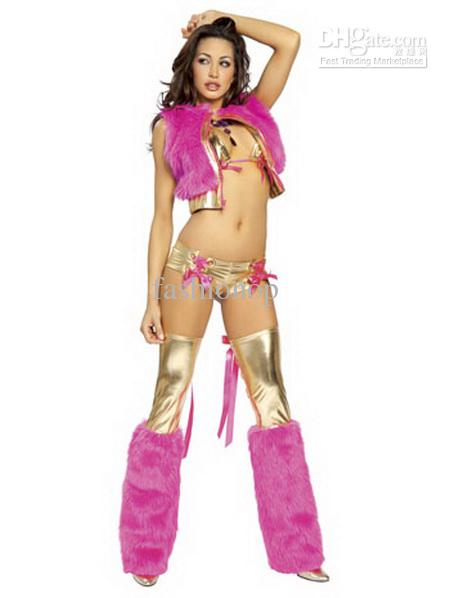
\includegraphics[scale=0.3]{socialmedia-memes/wear.jpg}
	\item <2->... don't share it!
	\end{itemize}
\end{frame}